\chapter{Практические задания}

\section*{Задание 1. Написать хвостовую рекурсивную функцию my-reverse, которая развернет верхний уровень своего списка-аргумента lst.}

\begin{lstinputlisting}[
	caption={Задание 1},
	label={lst:t1},
	style={lsp},
	linerange={1-6},
	]{../src/main.lsp}
\end{lstinputlisting}

\section*{Задание 2.  Написать функцию, которая возвращает первый элемент списка - аргумента, который сам является непустым списком.}

\begin{lstinputlisting}[
	caption={Задание 2},
	label={lst:t2},
	style={lsp},
	linerange={8-13},
	]{../src/main.lsp}
\end{lstinputlisting}

\section*{Задание 3.  Напишите рекурсивную функцию, которая умножает на заданное число-аргумент все числа из заданного списка-аргумента, когда}
a) все элементы списка --- числа,

б) элементы списка -- любые объекты.

\begin{lstinputlisting}[
	caption={Задание 3, a},
	label={lst:t3-1},
	style={lsp},
	linerange={24-30},
	]{../src/main.lsp}
\end{lstinputlisting}

\clearpage

\begin{lstinputlisting}[
	caption={Задание 3, b},
	label={lst:t3-2},
	style={lsp},
	linerange={32-37},
	]{../src/main.lsp}
\end{lstinputlisting}


\section*{Задание 4.Напишите функцию, select-between, которая из списка-аргумента, содержащего только числа, выбирает только те, которые расположены между двумя указанными границами-аргументами и возвращает их в виде списка (упорядоченного по возрастанию списка чисел (+ 2 балла))}

\begin{lstinputlisting}[
	caption={Задание 4},
	label={lst:t4},
	style={lsp},
	linerange={39-49},
	]{../src/main.lsp}
\end{lstinputlisting}

\section*{Задание 5. Написать рекурсивную версию (с именем rec-add) вычисления суммы чисел заданного списка:}
а) одноуровнего смешанного,

б) структурированного.

\begin{lstinputlisting}[
	caption={Задание 5, a},
	label={lst:t5-1},
	style={lsp},
	linerange={51-57},
	]{../src/main.lsp}
\end{lstinputlisting}

\begin{lstinputlisting}[
	caption={Задание 5, б},
	label={lst:t5-2},
	style={lsp},
	linerange={59-66},
	]{../src/main.lsp}
\end{lstinputlisting}


%\begin{figure}[h!]
%	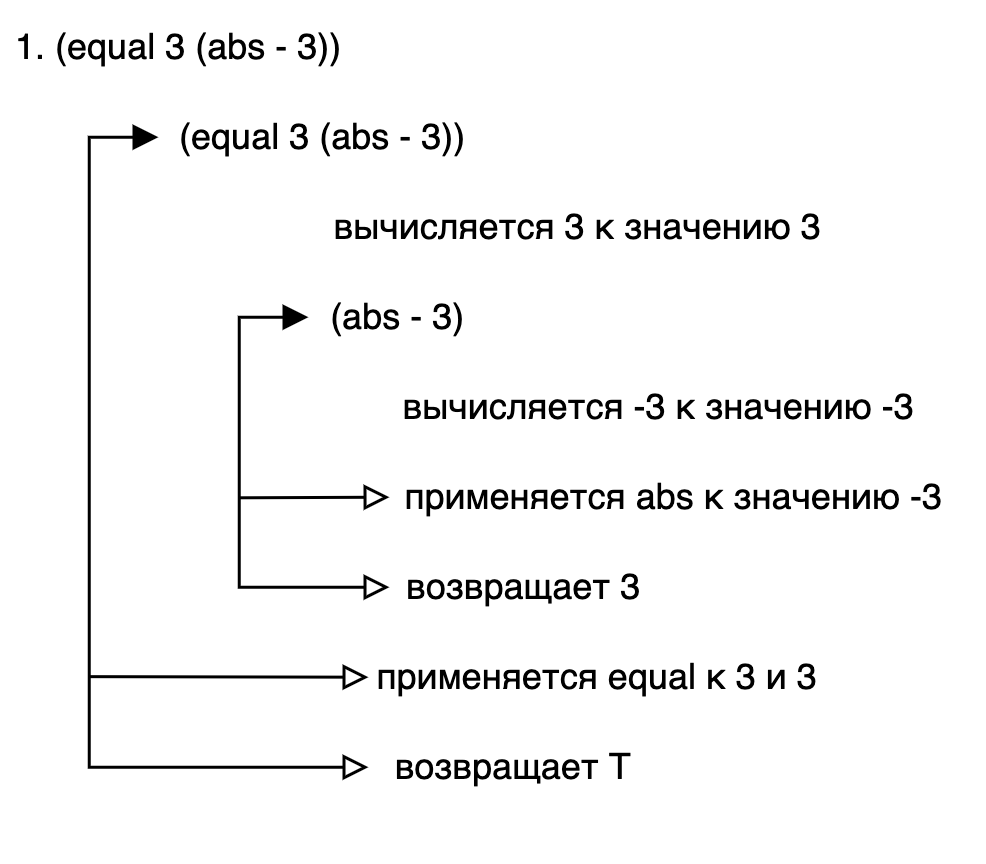
\includegraphics[scale=0.6,left]{task1.1}
%\end{figure}



